\chapter{解析結果}
本研究は,ゴルフスイングを数値化したデータに,ヒルベルト・ファン変換を適用させ,瞬時周波数領域で解析を行う.
\section{ゴルフスイングの数値化}
ゴルフスイングの数値化は,慣性式モーションキャプチャを使用して行う.
使用するモーションキャプチャは,PERCEPTION NEURON 2.0を使用する.
\begin{figure}
    \begin{center}
        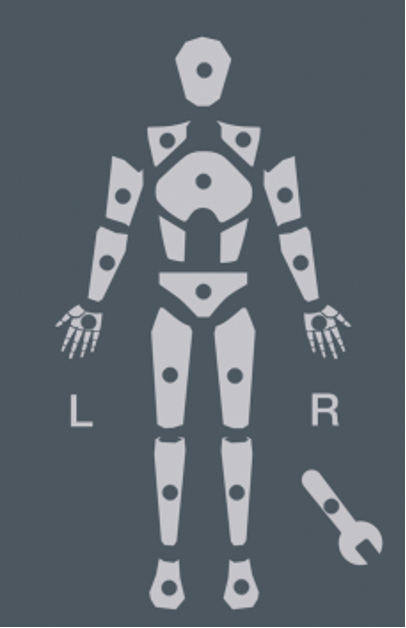
\includegraphics[width=3.5cm]{./images/sensors.png}
        \caption{加速度センサがついている位置}
        \label{sensors}
    \end{center}
\end{figure}
PERCEPTION NEURON 2.0は,図\ref{sensors}のように17点の位置に加速度センサを装着する.
この加速度センサより,推定の位置座標と$x$,$y$,$z$軸方向の回転角度を時系列にキャプチャしrawデータに書き出す.

PERCEPTION NEURON 2.0より,ゴルフスイングの時系列データを採取したrawデータであるため,bvh(biovision hierarchy)ファイルに変換する必要がある.
\begin{figure}
    \begin{center}
        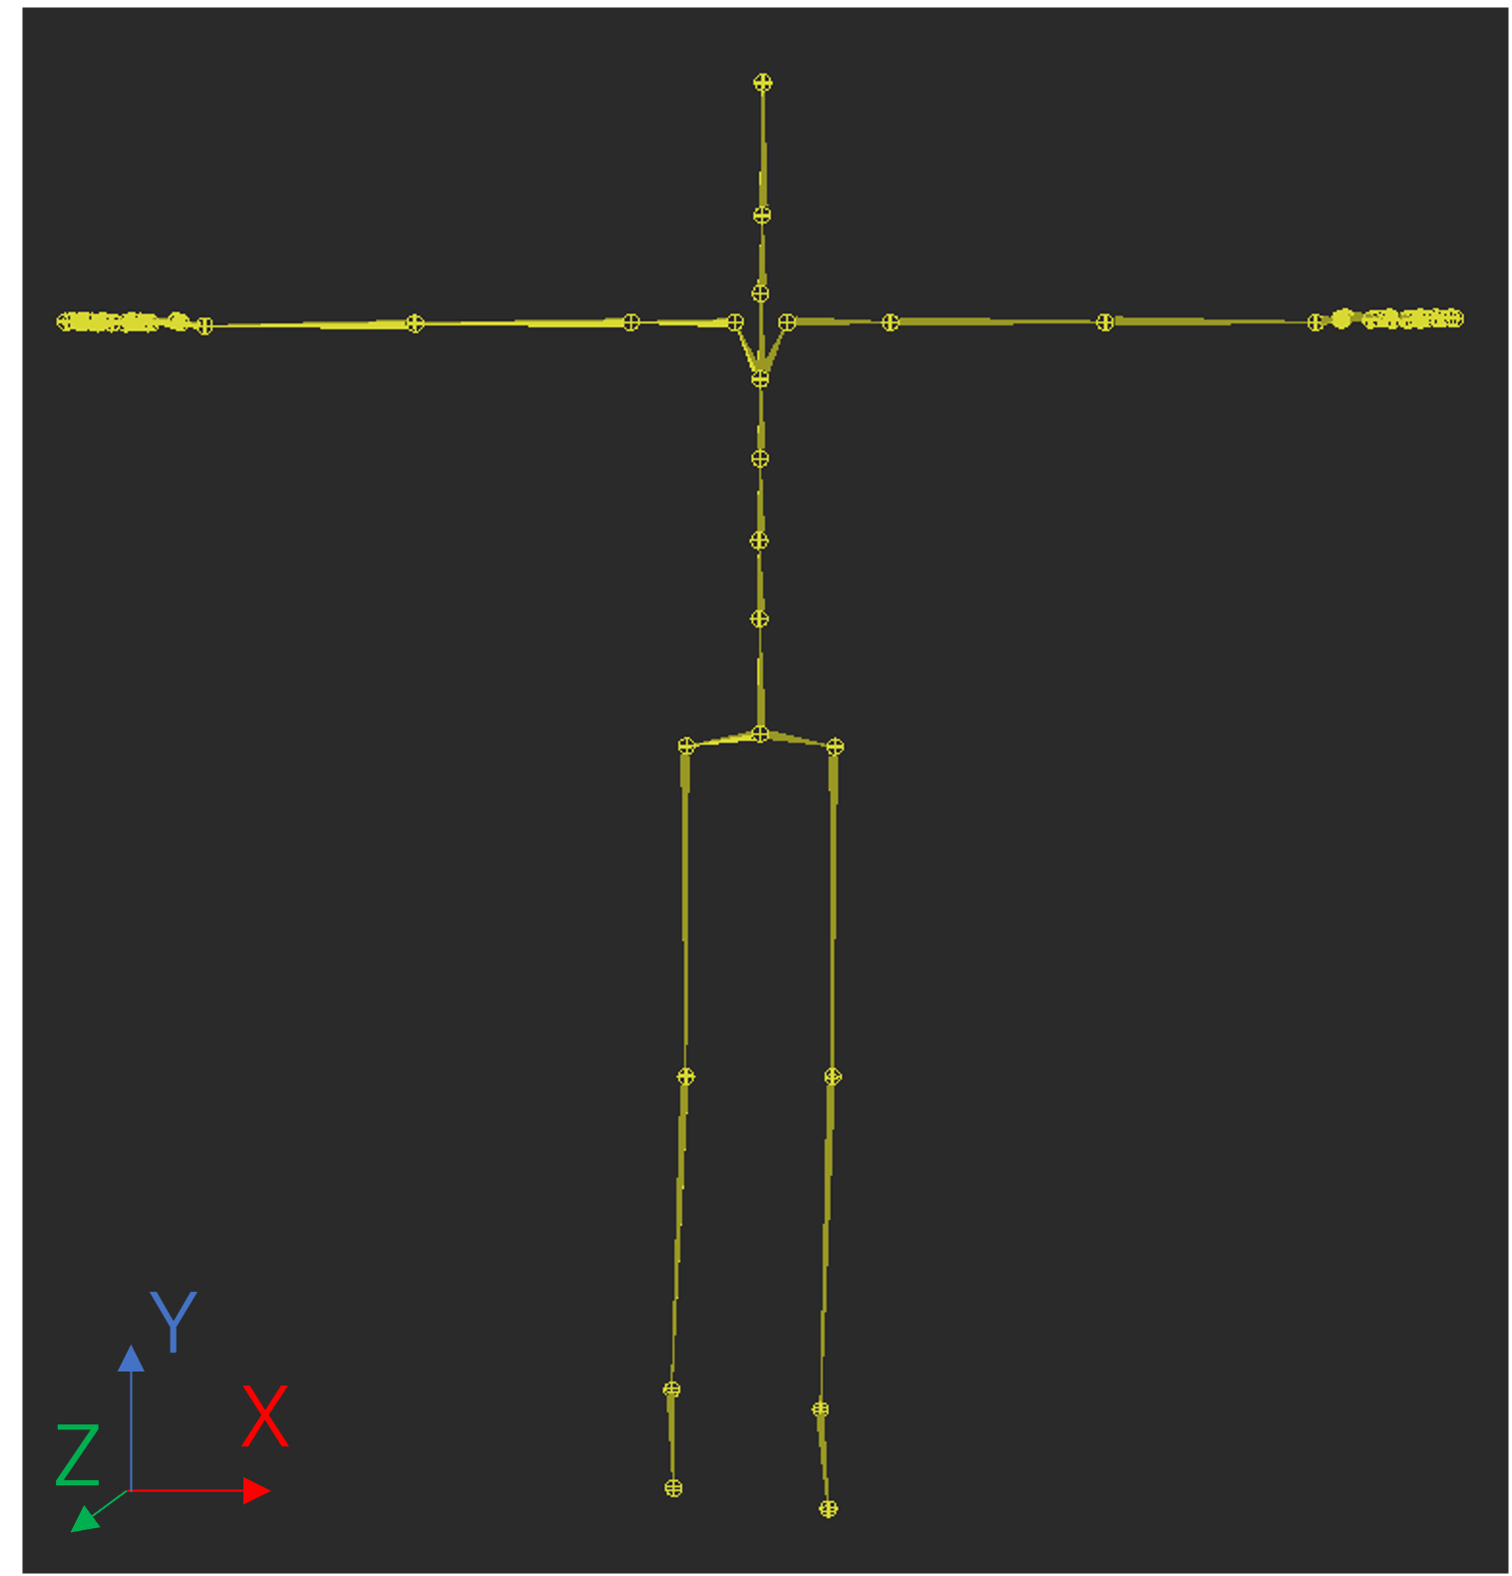
\includegraphics[width=5cm]{./images/Tpose.png}
        \caption{T-pose}
        \label{tpose}
    \end{center}
\end{figure}
bvhファイルとは,図\ref{tpose}のように指定された点の推定の位置座標や$x$,$y$,$z$軸方向の回転角を時系列に書き出したファイルである.
rawデータからbvhファイルの変換は,PERCEPTION NEURON 2.0専用ソフトであるAxis Neuronより行う.

図\ref{tpose}は,T-poseと呼ばれる,デフォルトポーズである.
このポーズより$x$,$y$,$z$軸方向を定義し,各関節球の$x$,$y$,$z$軸の回転角を0度とする.
bvhファイルに書き込まれている時系列データは,このポーズからの回転角を示し,ルートである腰部は$x$,$y$,$z$方向の位置座標も記録する.
よって,各関節球の3軸方向の回転角と腰部の3軸方向の位置座標を合計し,180チャンネルの時系列データを扱う.

\section{被験者情報}
ゴルフ歴10年のアベレージゴルファーがドライバーショットを打った.
被験者のドライバーショットでは,ストレート弾道のゴルフスイング,スライス弾道でヘッドアップ動作をしたゴルフスイング,スライス弾道で身体の開きの動作をしたゴルフスイングを6スイングずつ採取した.

本研究では,アベレージゴルファーのスライスの原因としてよく挙げられるヘッドアップ動作,身体が開く動作をしたゴルフスイングに注目し,ストレート弾道に飛球したゴルフスイングと比較して考察を行う.

\section{スペクトログラム解析}
\subsection{頸部,左膝モーションのIMF1}
\begin{figure}
    \begin{center}
        \begin{tabular}{c}
            \begin{minipage}{0.5\hsize}
                \begin{center}
                    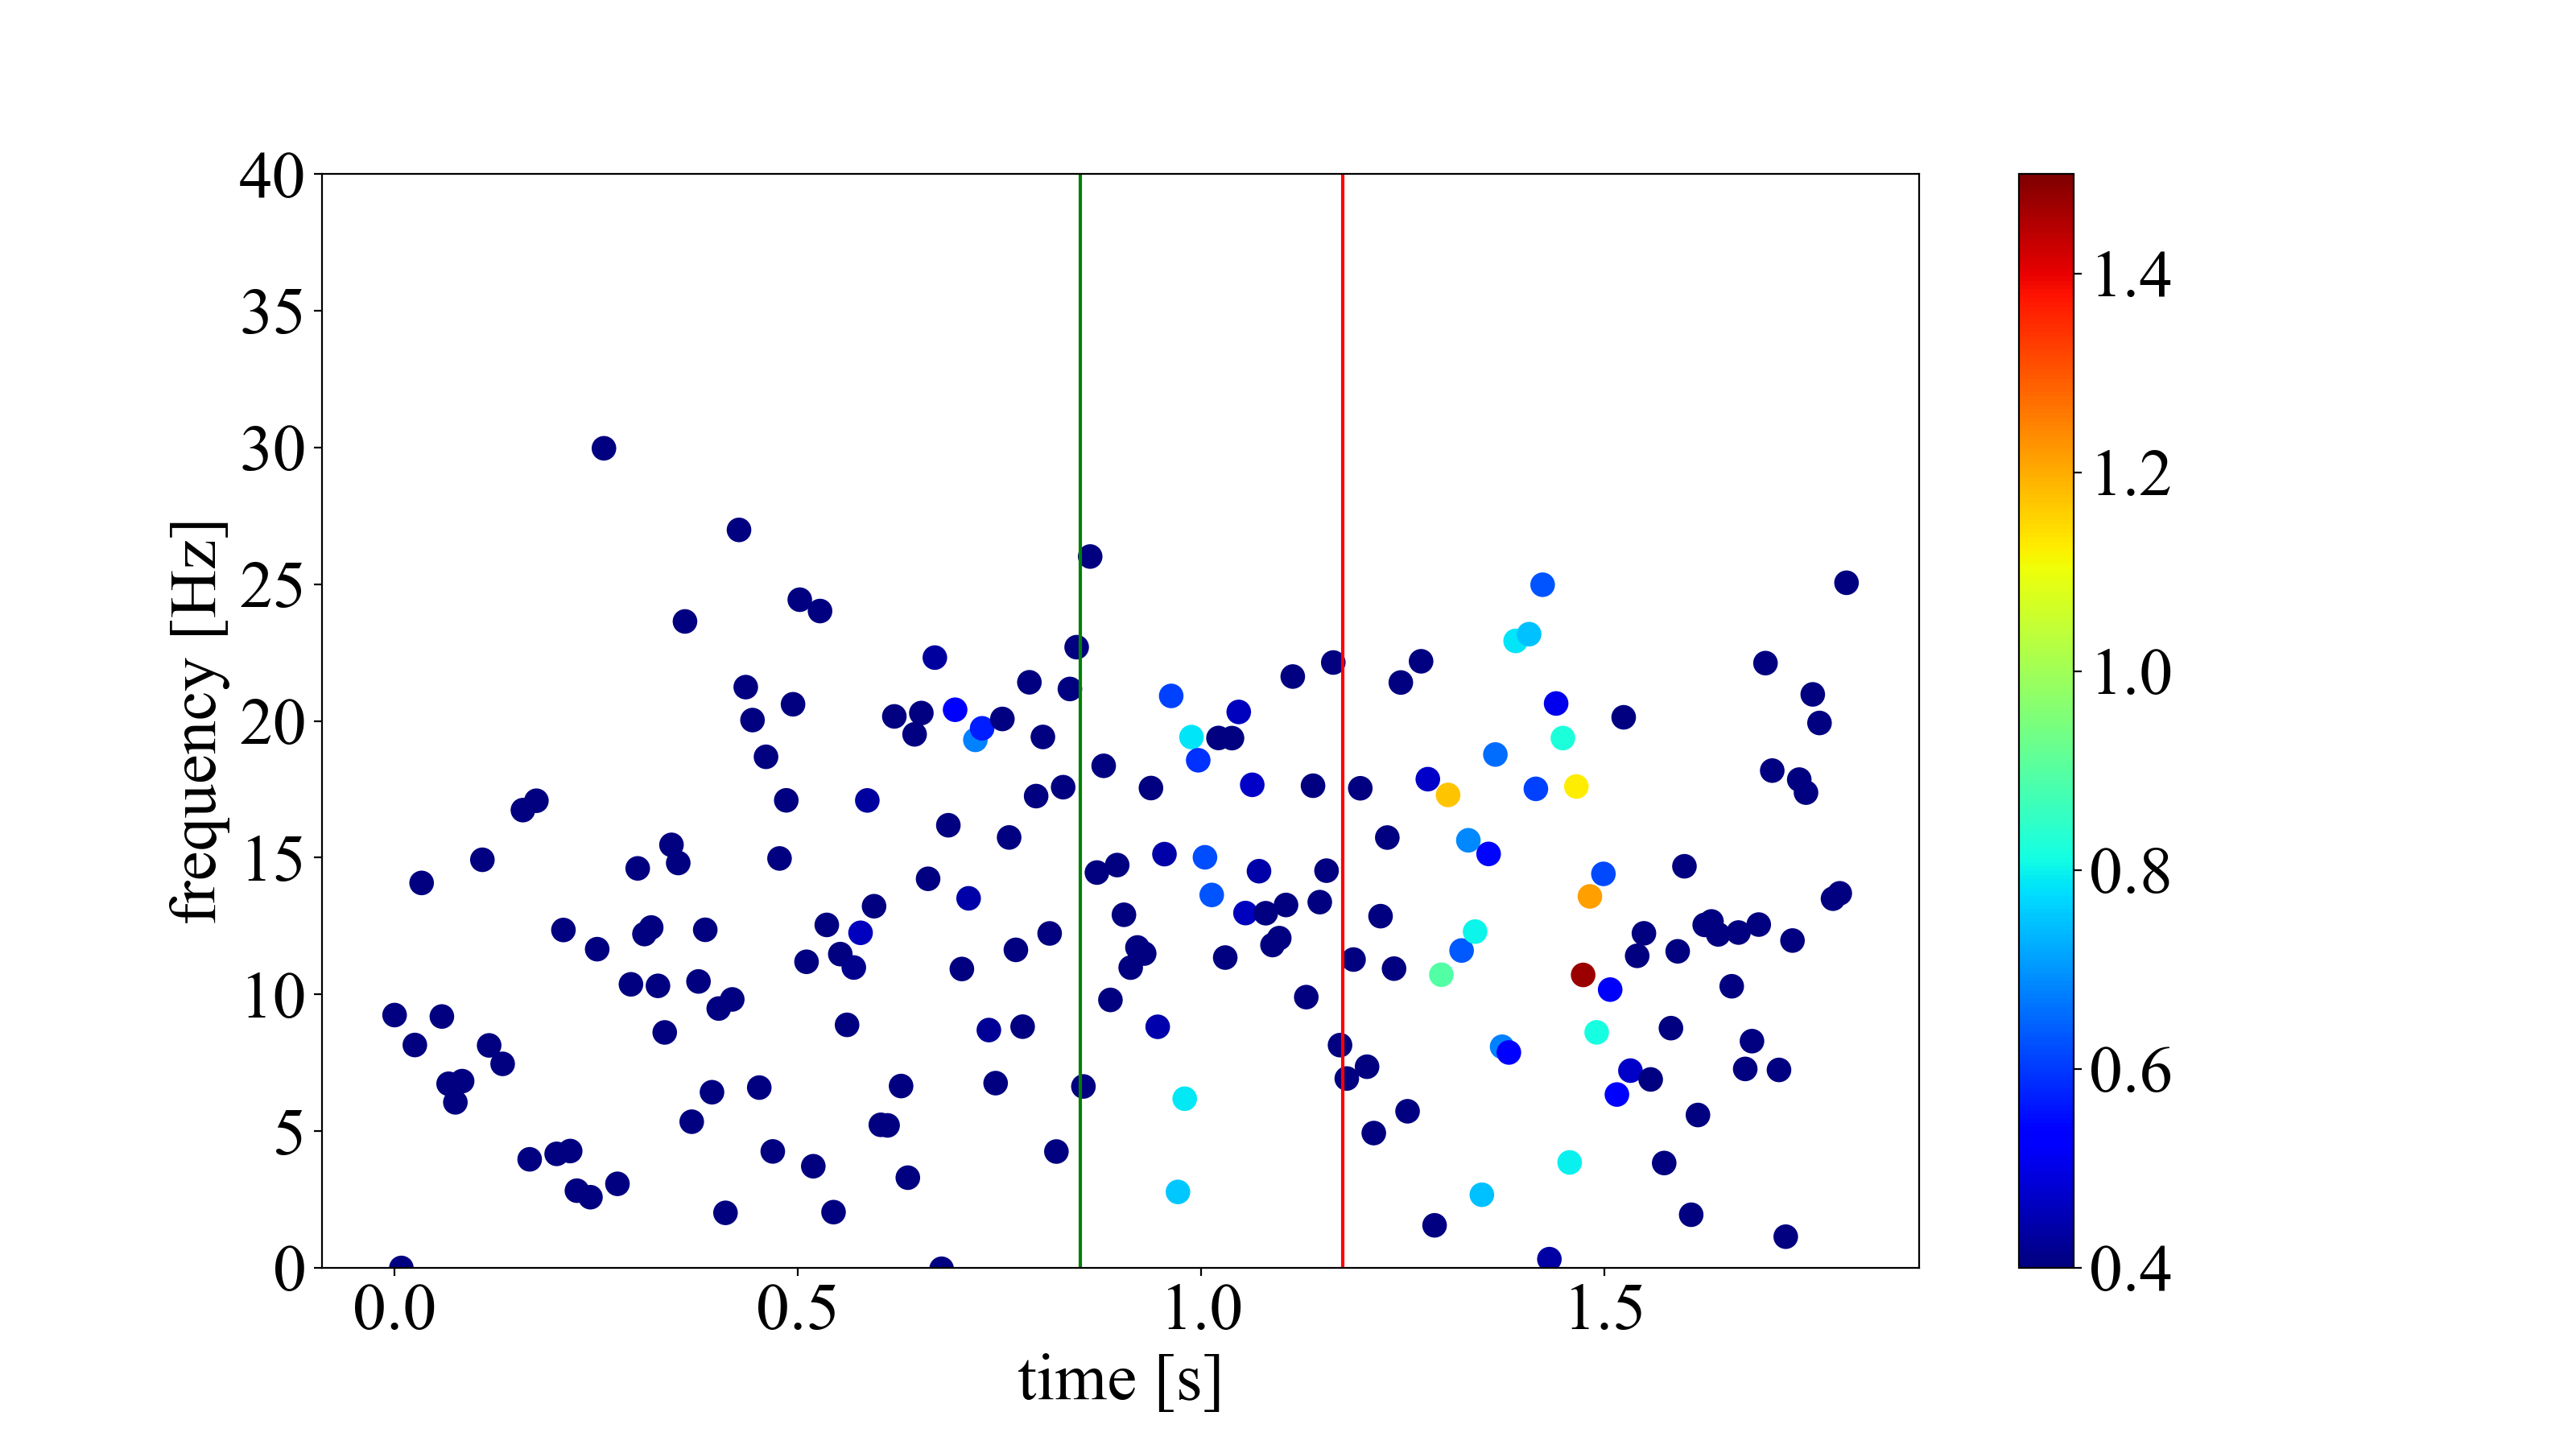
\includegraphics[width=8cm]{./images/straight_data/neck/IMF1.png}
                \end{center}
            \end{minipage}

            \begin{minipage}{0.5\hsize}
                \begin{center}
                    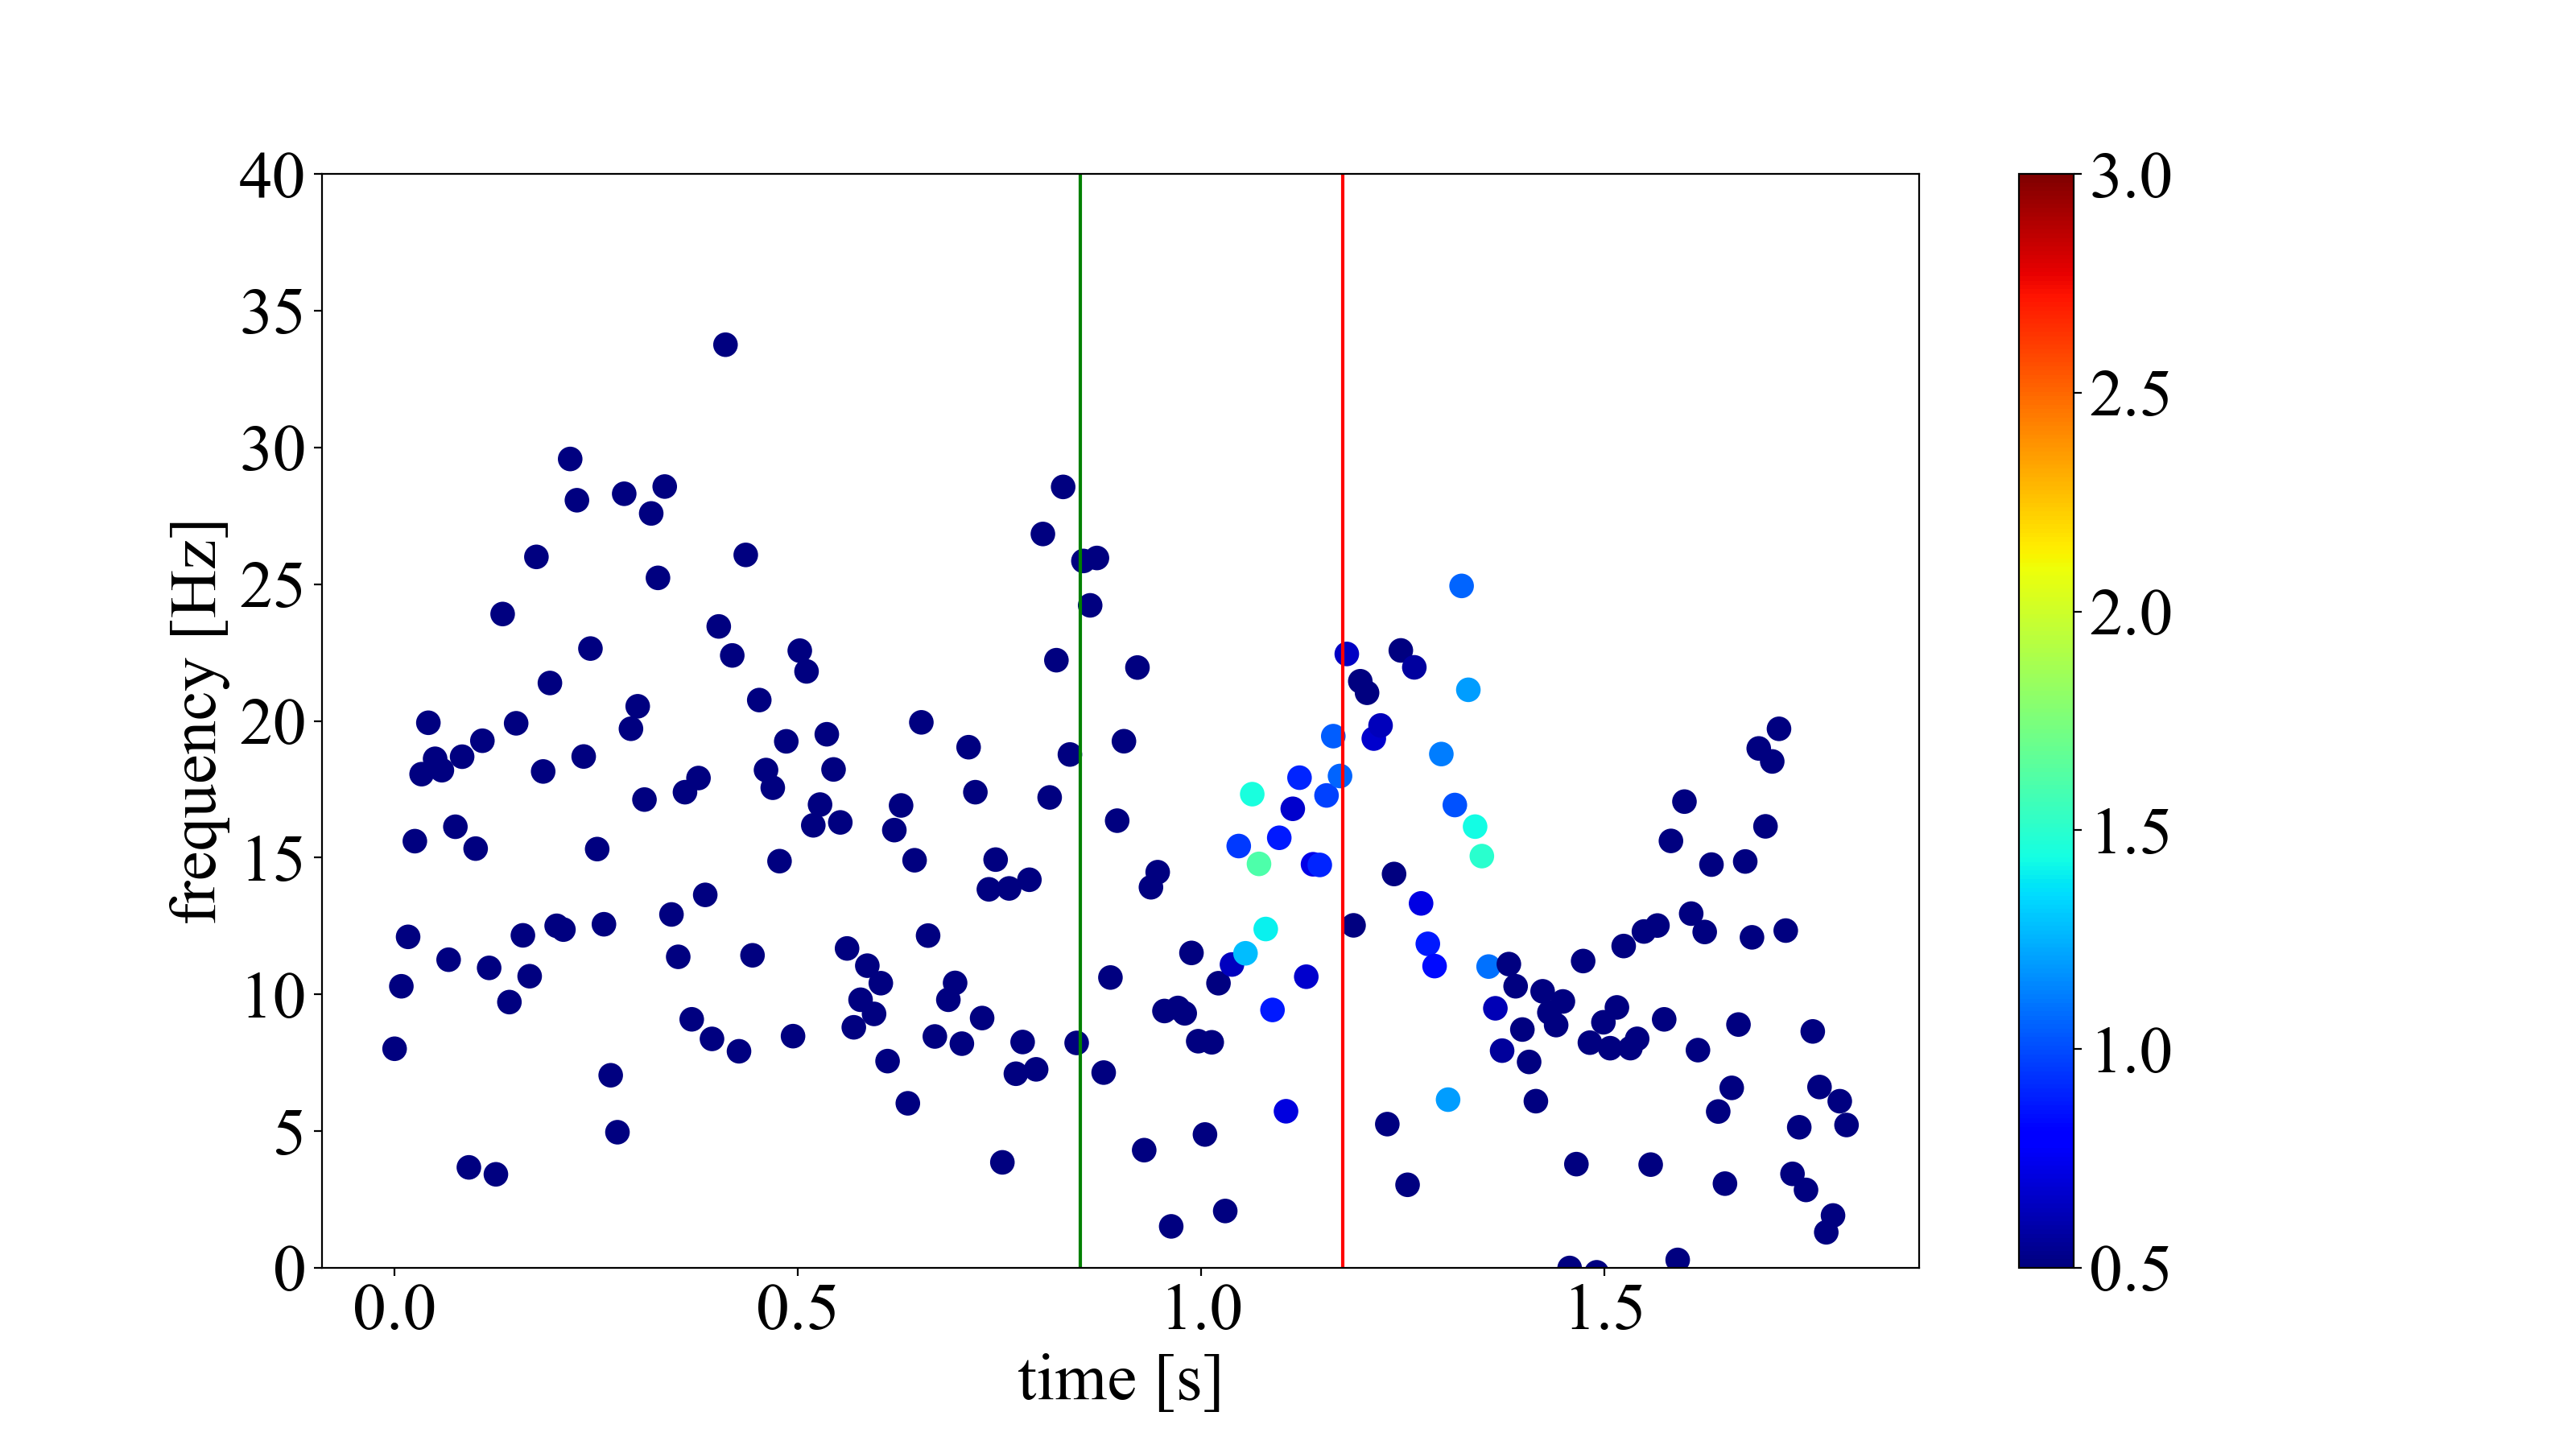
\includegraphics[width=8cm]{./images/straight_data/left_leg/IMF1.png}
                \end{center}
            \end{minipage}
        \end{tabular}
    \end{center}
\end{figure}

\begin{figure}
    \begin{center}
        \begin{tabular}{c}
            \begin{minipage}{0.5\hsize}
                \begin{center}
                    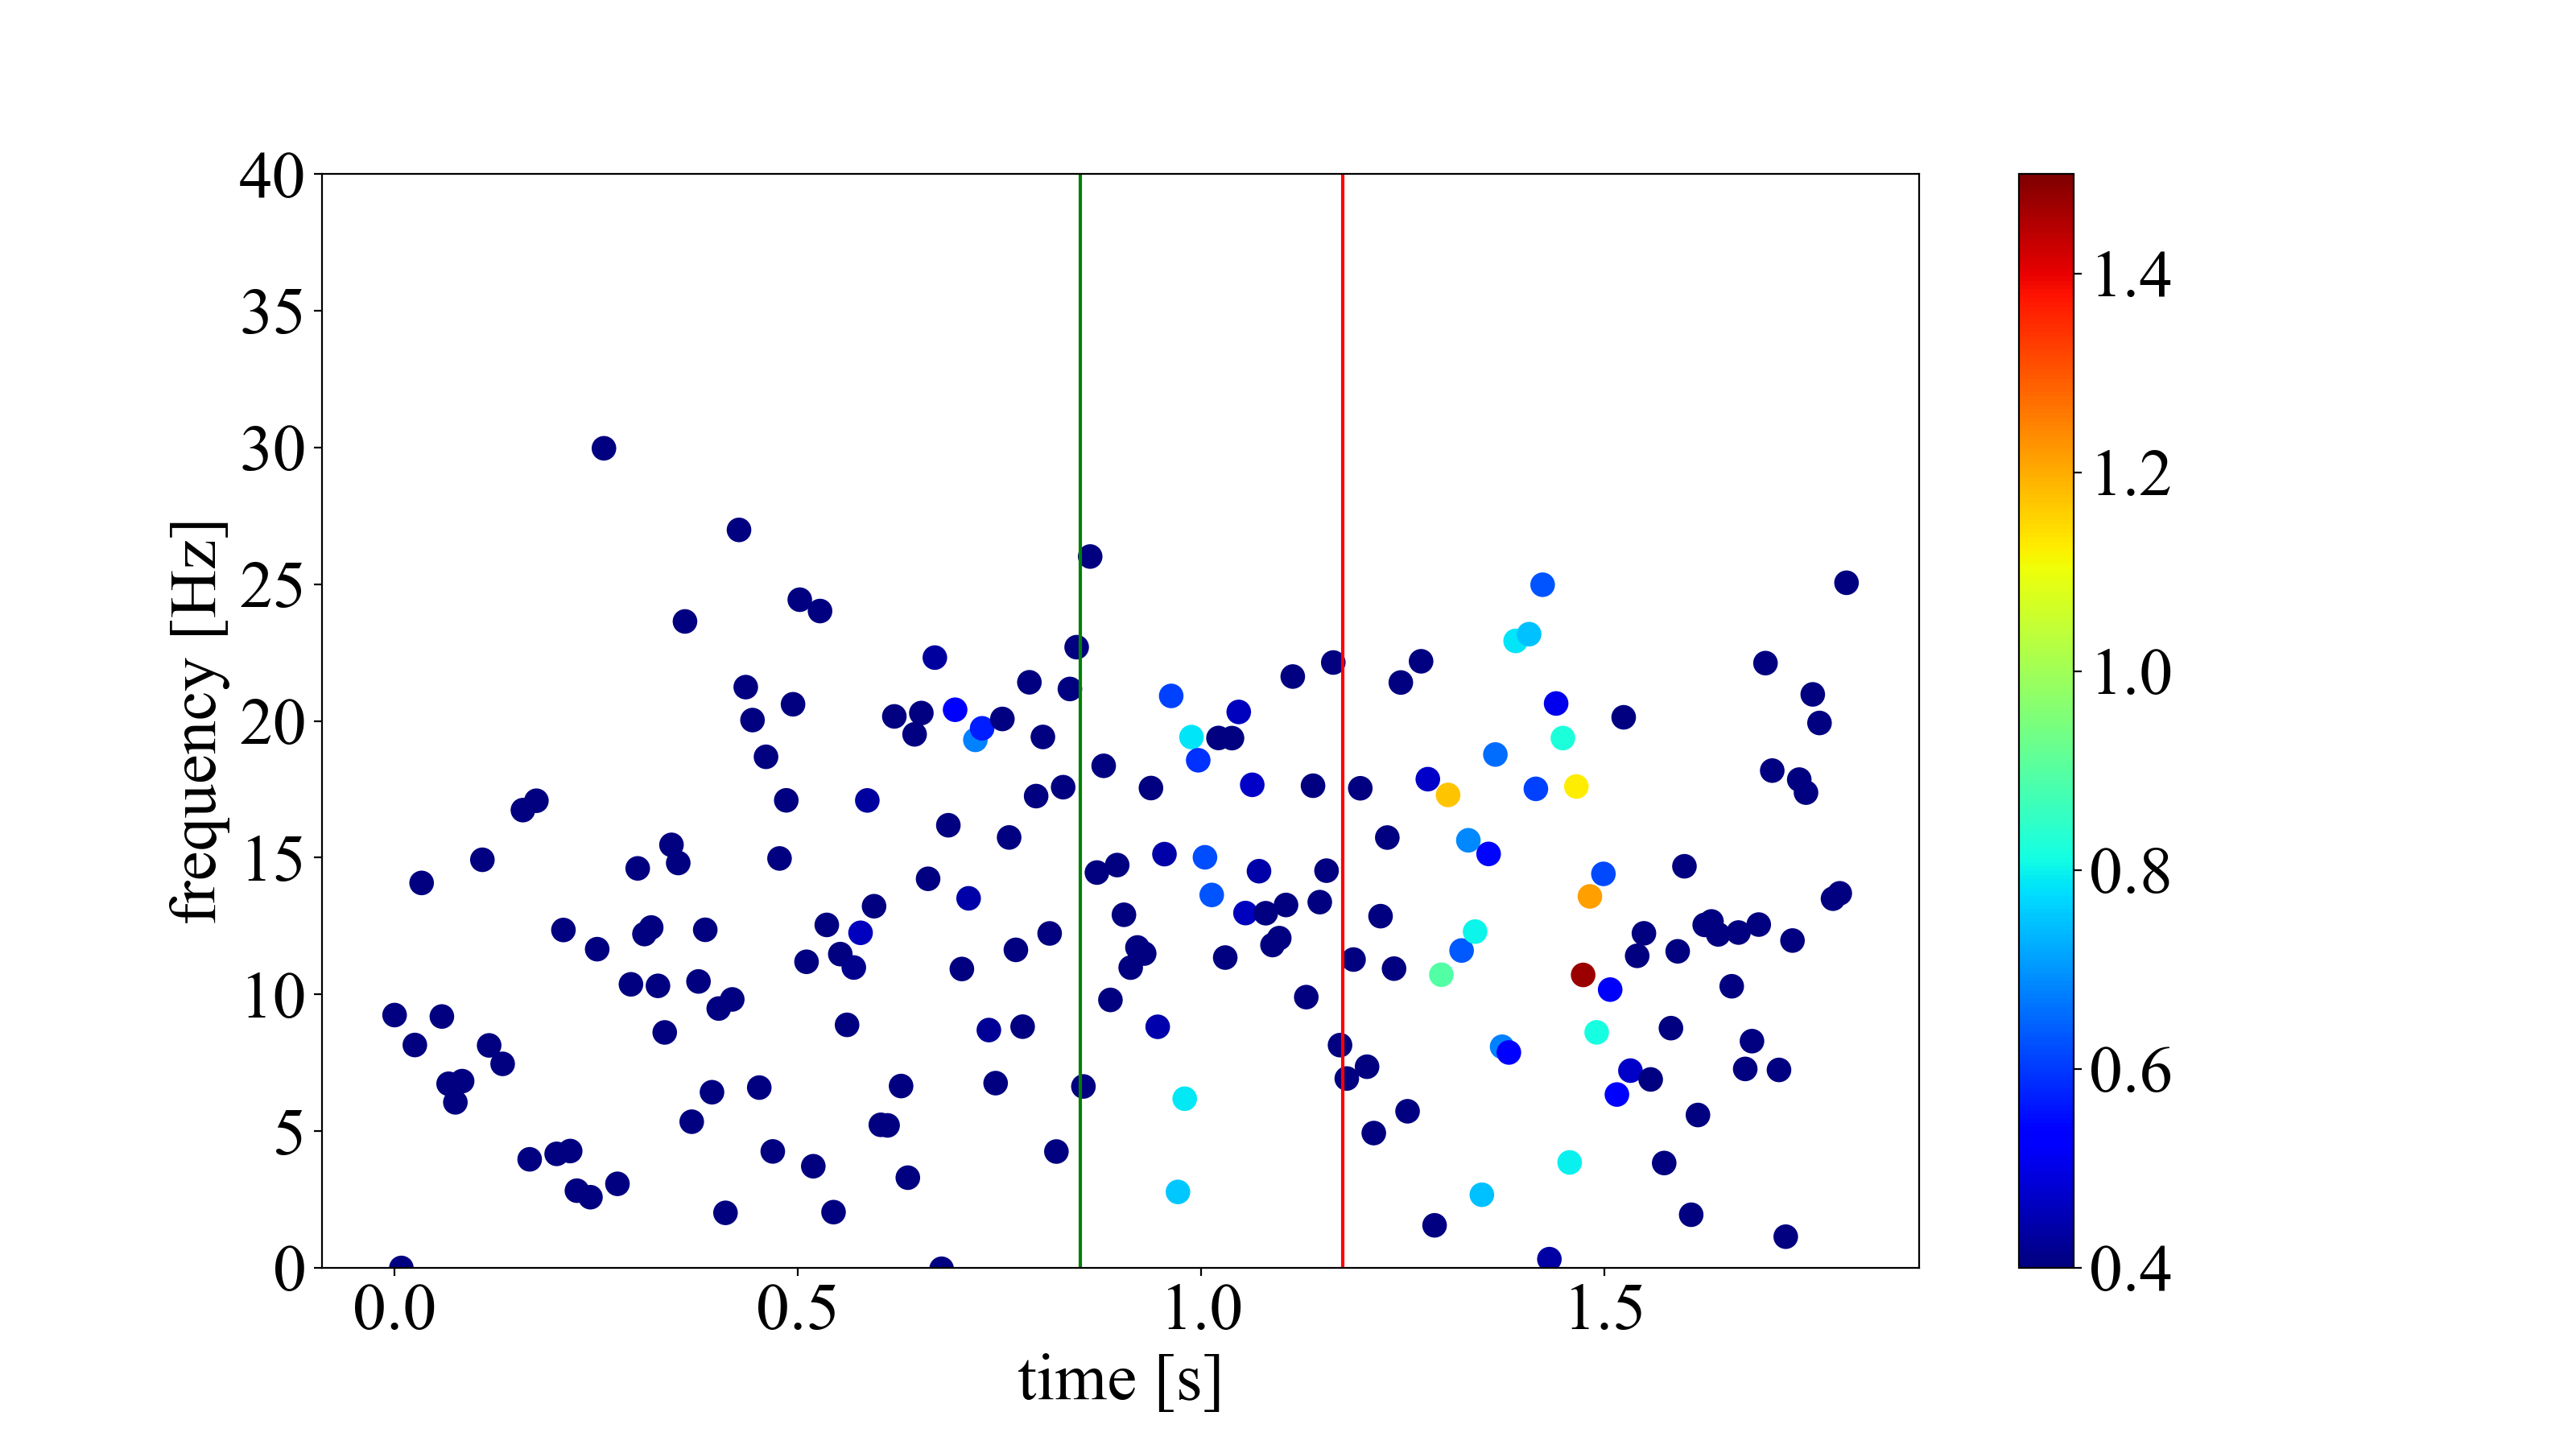
\includegraphics[width=8cm]{./images/straight_data/neck/IMF1.png}
                \end{center}
            \end{minipage}

            \begin{minipage}{0.5\hsize}
                \begin{center}
                    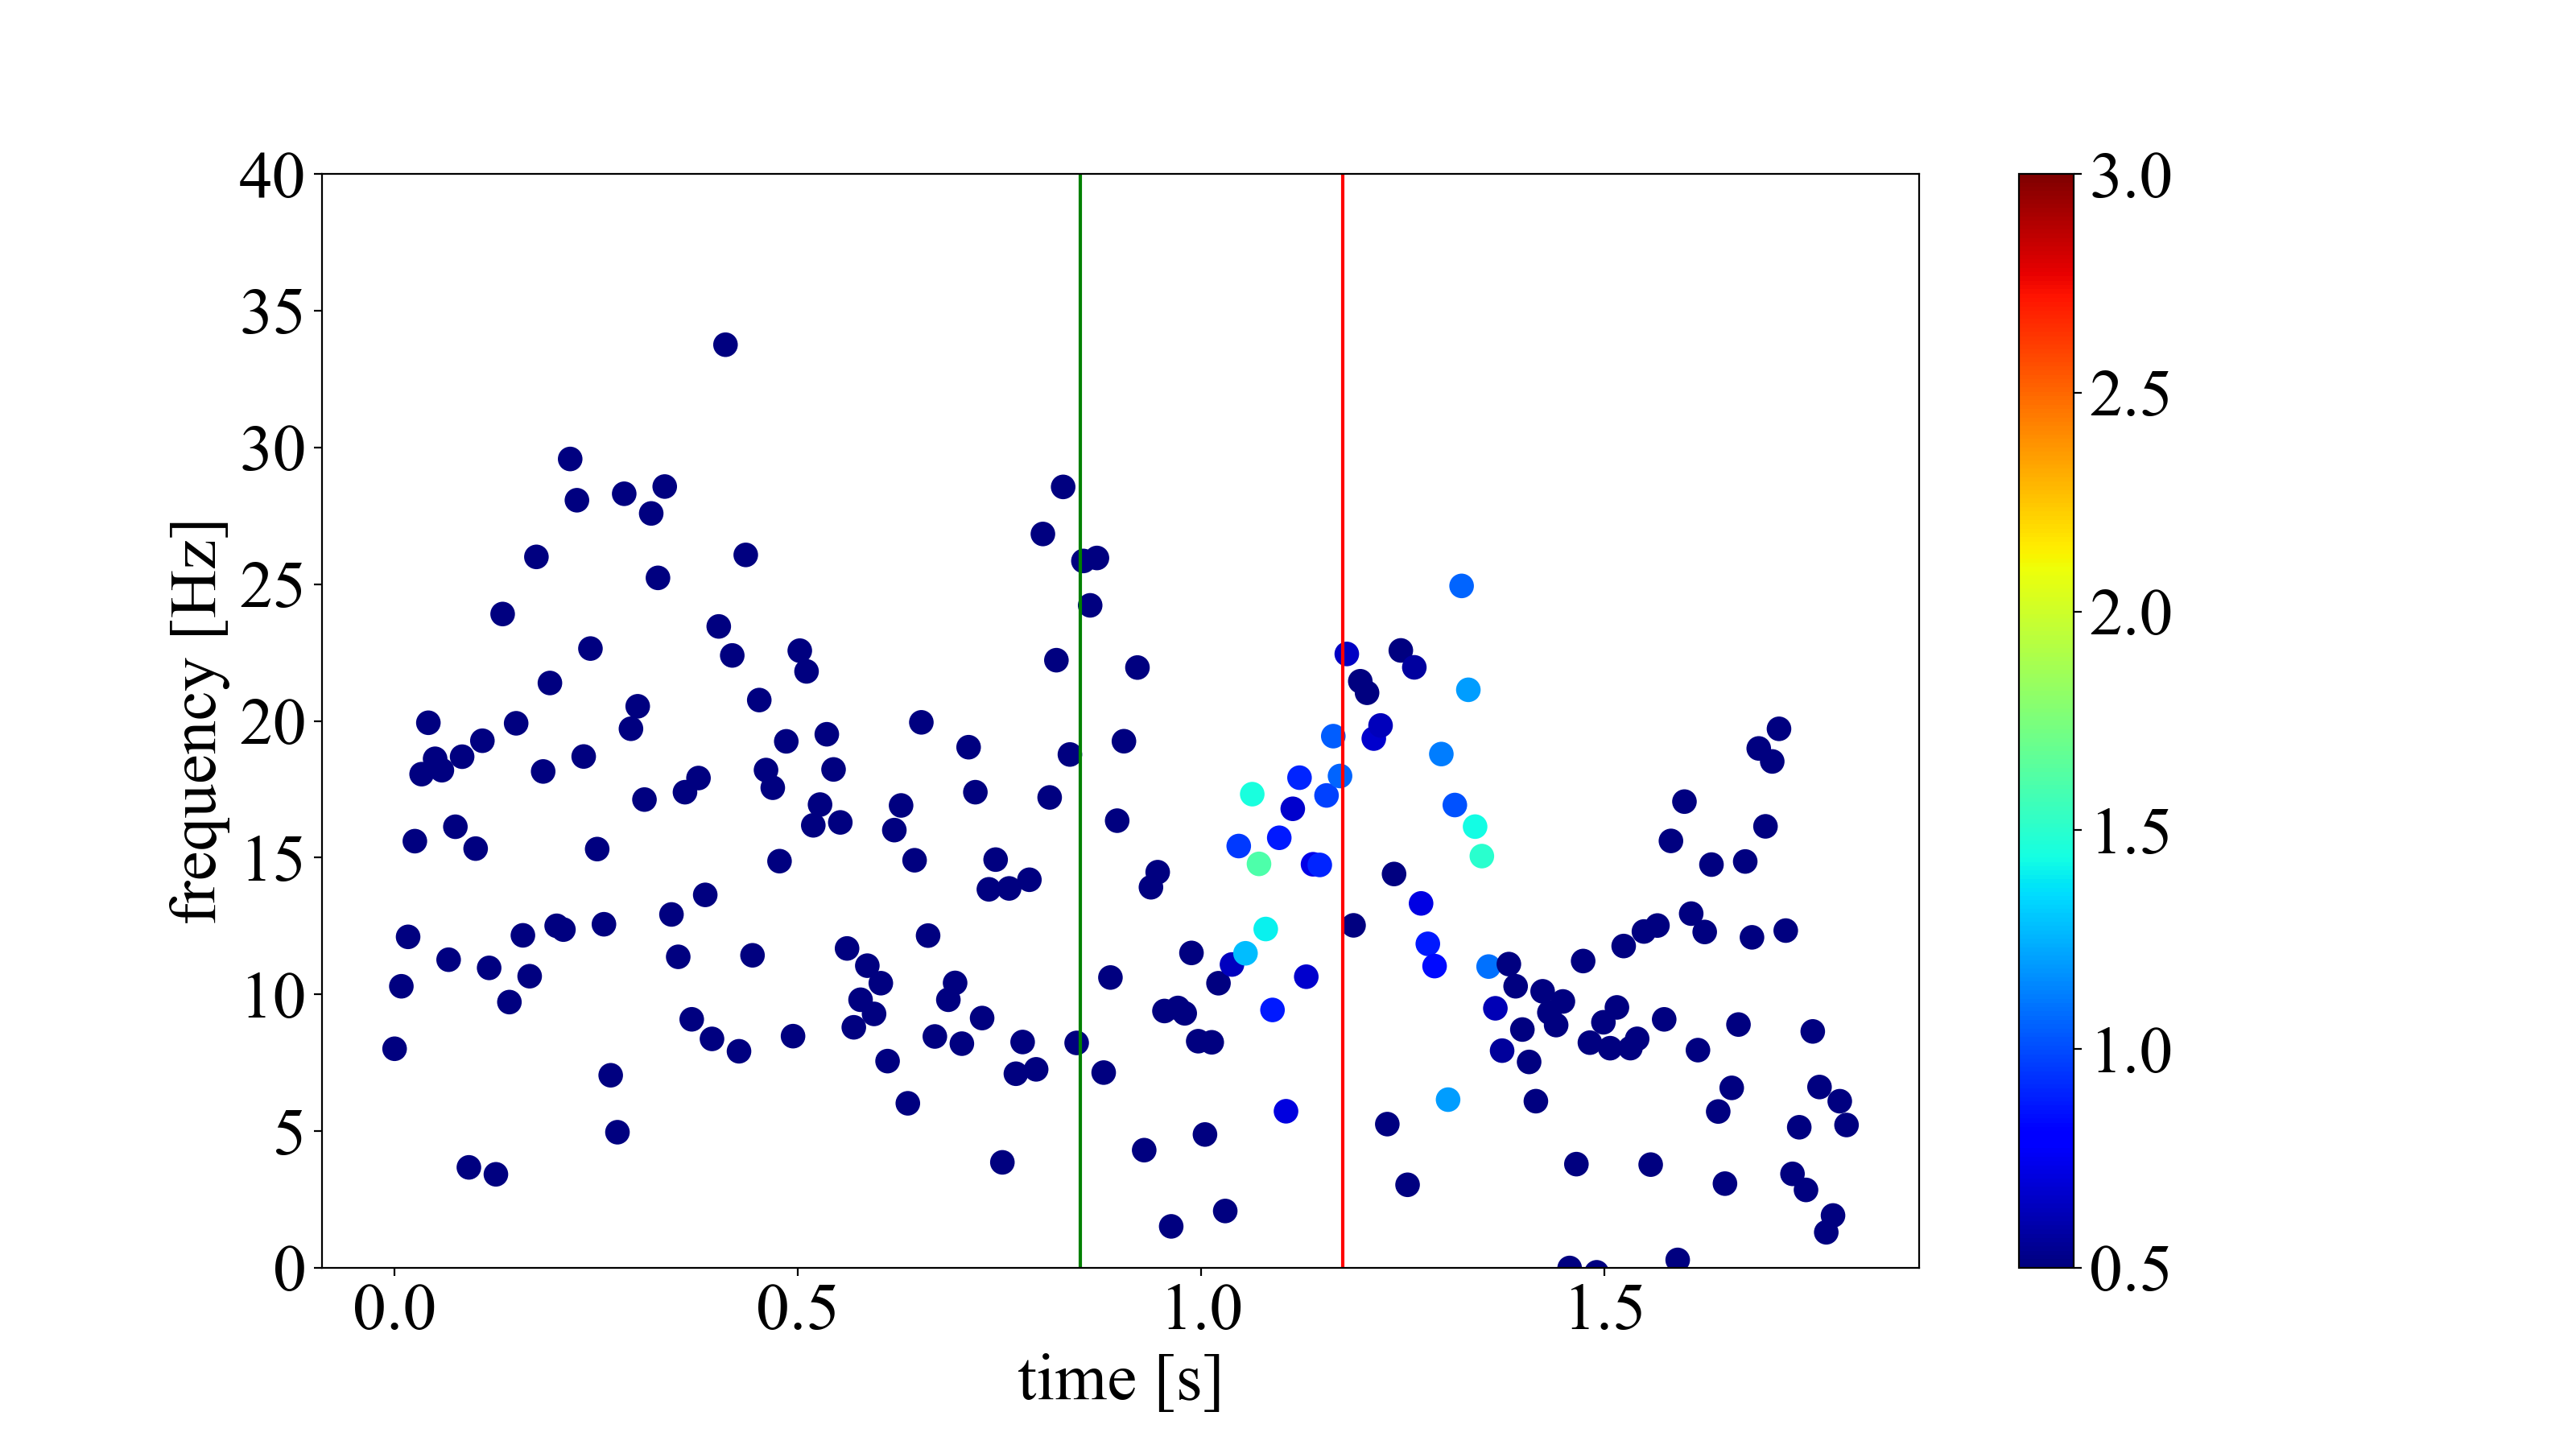
\includegraphics[width=8cm]{./images/straight_data/left_leg/IMF1.png}
                \end{center}
            \end{minipage}
        \end{tabular}
    \end{center}
\end{figure}

\subsection{頸部,左膝,左腿モーションのIMF4}